\section{Experimentación}
\subsection{Protocolo de validación}
\begin{frame}
  \frametitle{Protocolo de validación}
\begin{figure}[htp]
 \begin{center}
   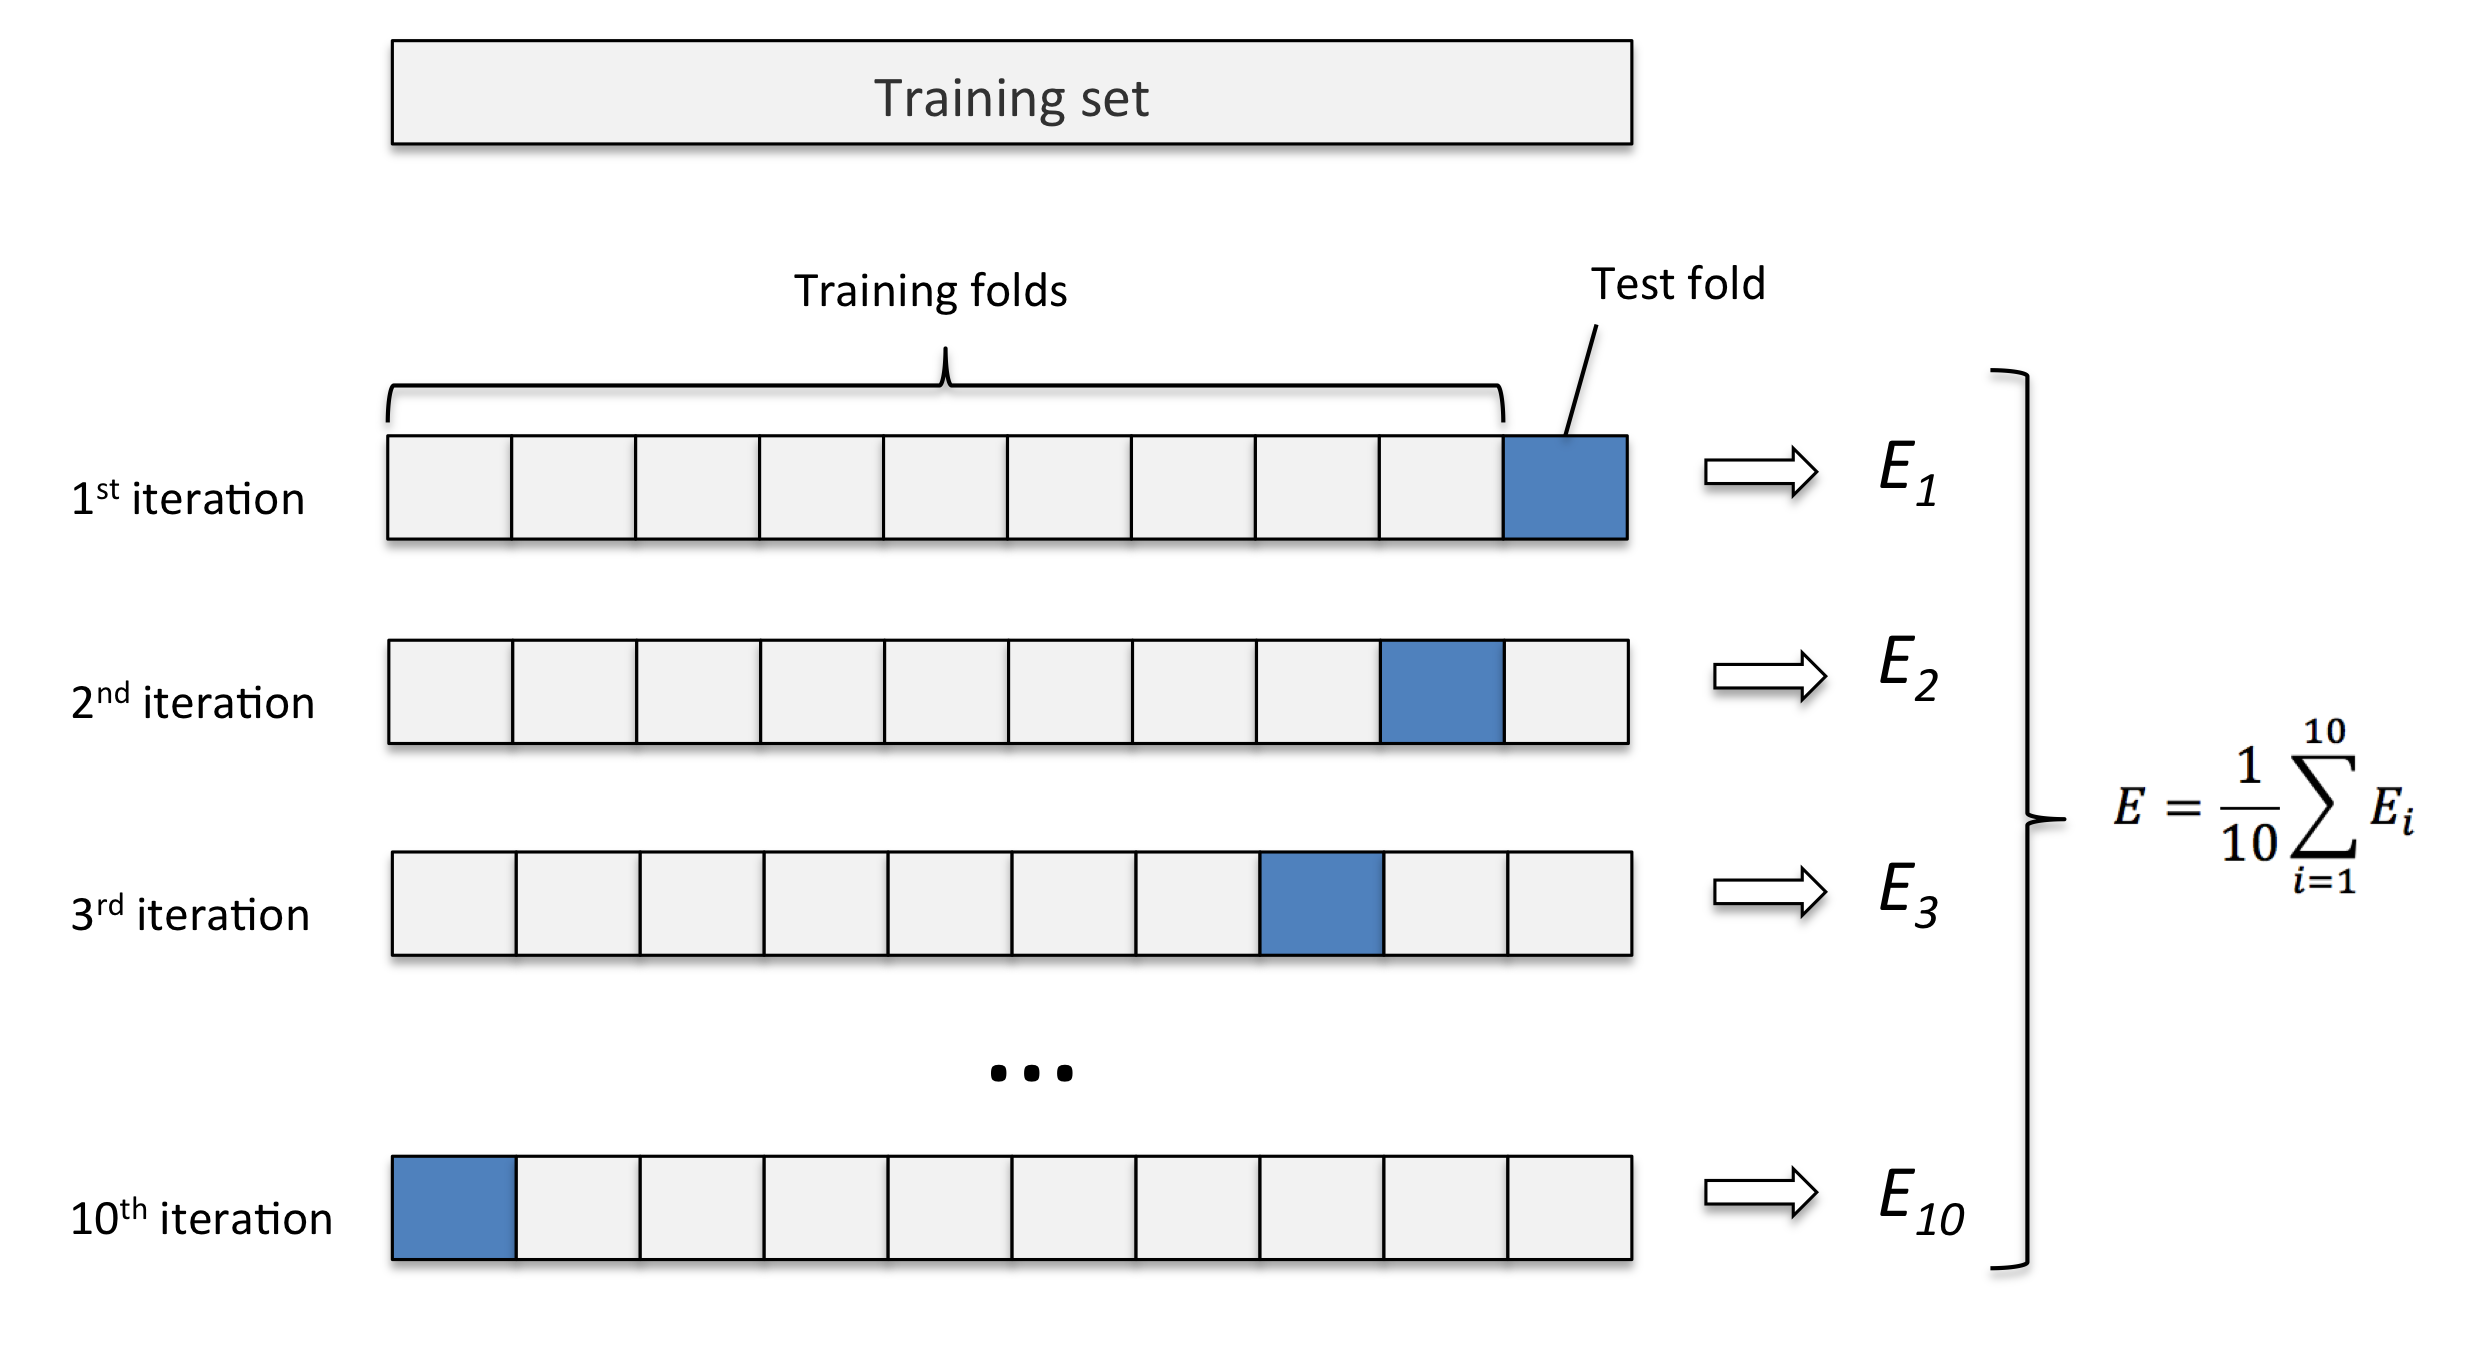
\includegraphics[width=.8\textwidth]{imagenes/chapter4/cross-validation}
 \end{center}
\end{figure}

\end{frame}

\subsection{Modelo NR3DQA}
\begin{frame}
  \frametitle{Modelo NR3DQA\footnotemark[11]}
\begin{table}[htp]
  \small
  \begin{center}
    \begin{tabular}[c]{|c|c|c|c|c|}
      \hline
      \rowcolor[HTML]{FFC702}
      \textbf{Dataset} & \textbf{PLCC} & \textbf{SROCC} & \textbf{KROCC} \\ 
      \hline
      SJTU & \textbf{0.810325} & \textbf{0.777403} & \textbf{0.608302} \\ 
      \hline 
      WPC & 0.637953 & 0.634853 & 0.463578 \\
      \hline
    \end{tabular}
  \end{center}
  \caption[Resultados de prueba preliminar con SVM.]{Replicando experimentos de Zhang et al\footnotemark[11].}
  \label{tab:PlainNR3DQA}
\end{table}
\begin{table}[htp]
  \small
  \begin{center}
    \hspace{-.5cm}
    \begin{tabular}[c]{|c|c|c|c|c|}
      \hline
      \rowcolor[HTML]{FFC702}
      \multicolumn{1}{|c|}{\textbf{Etiqueta Sintética}} & 
      \multicolumn{1}{|c|}{\textbf{Modelo}} & 
      \multicolumn{1}{|c|}{\textbf{Escalado}} & 
      \multicolumn{1}{|c|}{\textbf{PLCC}} &
      \multicolumn{1}{|c|}{\textbf{SROCC}} \\
      \hline
      Valor de la métrica & SVM & RobustScaler & 0.2017 & 0.1776 \\
      \hline
      Valor normalizado & KNNRegressor & RobustScaler & 0.2671 & 0.1882  \\
      \hline
      Valor en escala 0-5 & DecisionTree & StandardScaler & \textbf{0.309176} & \textbf{0.196713} \\
      \hline
    \end{tabular}
  \end{center}
  \caption[Resultados de prueba preliminar con NR3DQA.]{
    Resultados de prueba preliminar con NR3DQA\footnotemark[11]. 
  }
  \label{tab:MedicalNR3DQA}
\end{table}
\footnotetext[11]{\cite{NR3DQA}}

\end{frame}

\begin{frame}
  \frametitle{Modificaciones}
  \begin{columns}
    \column{0.5\textwidth}
    \begin{itemize}
      \item Weinmann et al\footnotemark ~estudiaron los procesos de: 
        \begin{itemize}
          \item Segmentación.
          \item Detección.
          \item Clasificación.
        \end{itemize}
      \item Justifican la importancia de:  
        \begin{itemize}
          \item Omnivarianza.
          \item Entropía de los valores singulares.
          \item Verticalidad del vecindario.
        \end{itemize}
    \end{itemize}
    \column{0.5\textwidth}
  \begin{table}[htp]
    \small
    \begin{center}
      \begin{tabular}[c]{|c|c|c|c|c|}
        \hline
        \rowcolor[HTML]{FFC702}
        \textbf{Dataset} & \textbf{PLCC} & \textbf{SROCC} & \textbf{KROCC} \\ 
        \hline
        SJTU & \textbf{0.853709} & \textbf{0.820057} & \textbf{0.649406} \\ 
        \hline 
        WPC & 0.642356 & 0.62917 & 0.455562 \\
        \hline 
        Nuestro & 0.344601 &  0.170793 & -- \\
        \hline
      \end{tabular}
    \end{center}
    \caption[Resultado de mejoras sobre el método SVM]{Resultado de mejoras sobre el método SVM.}
    \label{tab:ImprovNR3DQA}
  \end{table}
\end{columns}
\footcitetext{3DNSSMetrics}
\end{frame}


\subsection{Modelo VQA-PC}
% \begin{frame}
%   \frametitle{Hiperparámetros del modelo VQA-PC\footnotemark[12]}
%   \begin{table}[htp]
%     \small
%     \begin{center}
%       \begin{tabular}[c]{|c|c|}
%         \hline
%         \rowcolor[HTML]{FFC702}
%         \textbf{Hiperparámetro} & \textbf{Valor} \\ 
%         \hline 
%         Tasa de aprendizaje &  0.0004 \\ 
%         \hline 
%         Tamaño de batches & 32 \\ 
%         \hline 
%         Tasa de decadencia & 0.9 \\ 
%         \hline 
%         Frecuencia de decadencia & 10 \\ 
%         \hline 
%         Épocas & 30 \\ 
%         \hline 
%         K-fold & 9 \\ 
%         \hline 
%       \end{tabular}
%     \end{center}
%     \caption[Hiperparámetros empleados en la experimentación preliminar.]{
%       Hiperparámetros empleados en la experimentación preliminar\footnotemark[12]
%     }
%       \vspace{-.6cm}
%     \label{tab:HiperSJTU}
%   \end{table}
%   \footnotetext[12]{\cite{VQA-PC}}
% \end{frame}
%
\begin{frame}
  \frametitle{Experimentos preliminares VQA-PC}
\begin{table}[htp]
  \small
  \begin{center}
    \begin{tabular}[c]{|c|c|c|}
      \hline
      \rowcolor[HTML]{FFC702}
      \textbf{Kfold} & \textbf{MSE} & \textbf{SROCC} \\ 
      \hline 
      0 & 13.9222 & 0.8995 \\
      \hline 
      1 & 418120.5625 & 0.8547 \\ 
      \hline 
      2 & 10.9271 & 0.9081 \\
      \hline 
      3 & 19.8226 & 0.9295 \\ 
      \hline 
      4 & 443.6077 & 0.8700 \\ 
      \hline 
      5 & 28.3165 & 0.9544 \\ 
      \hline 
      6 & 292.239 & 0.7675 \\ 
      \hline 
      7 & 329.0685 & 0.8833 \\ 
      \hline 
      8 & 357.0455 & 0.8647 \\ 
      \hline
      \textbf{\cellcolor[HTML]{FFC702}Promedio} & \textbf{46623.94} & \textbf{0.8813} \\ 
      \hline
    \end{tabular}
  \end{center}
  \caption[Resultados de experimento preliminar.]{
    Resultados de experimento preliminar. 
  }
  \label{tab:PreTestResults}
\end{table}
\end{frame}

\begin{frame}
  \frametitle{Curvas de aprendizaje VQA-PC}
  \vspace{-.2cm}
\begin{figure}[htp]
  \centering
    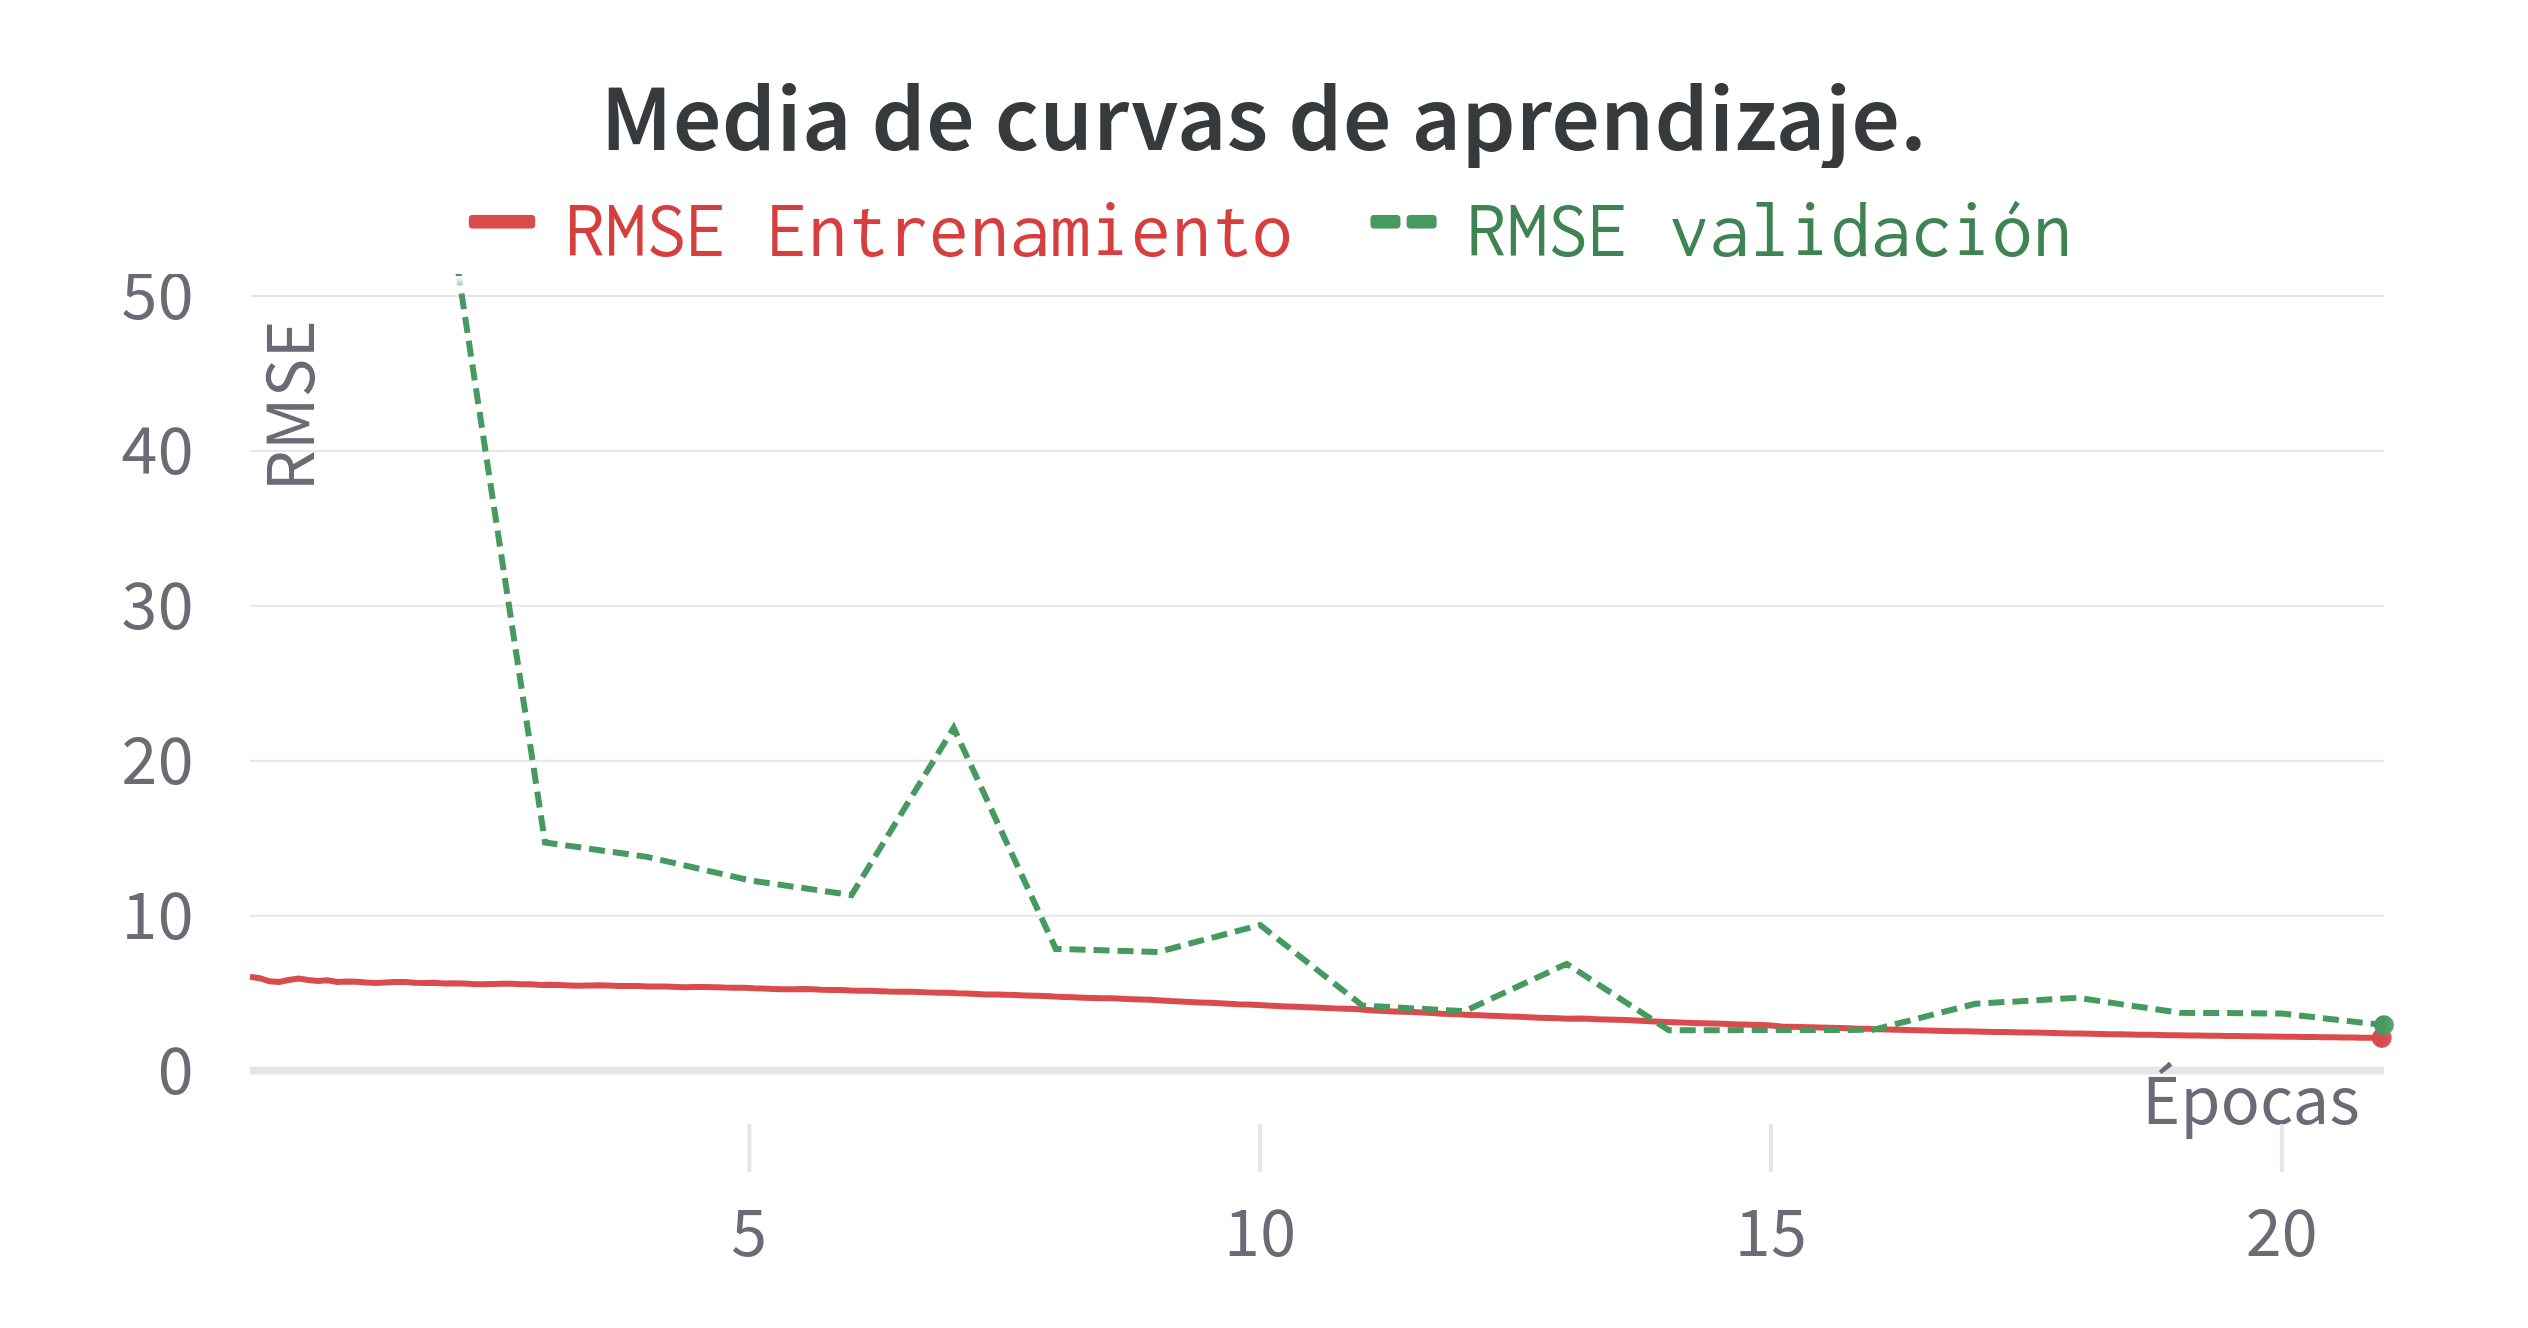
\includegraphics[width=.75\textwidth]{imagenes/chapter4/PreTestCurves.png}
  \caption[Curvas de aprendizaje del test preliminar.]{
    Curvas de aprendizaje del test preliminar. 
  } 
\label{fig:PreTestCurves}
\end{figure}
\end{frame}

\begin{frame}
  \frametitle{Modificaciones}
  \begin{enumerate}
    \item Abouelaziz et al\footnotemark~ experimentaron \textbf{distintos métodos de fusión de características}.
      \begin{itemize}
        \item Fusión por \textbf{concatenación} (F0).
        \item Fusión por \textbf{multiplicación} (F1). 
        \item Fusión por \textbf{convolución 1x1} (F2).
        \item Fusión por \textbf{\emph{compact multi-linear pooling}} (F3).
      \end{itemize}
    \item Experimentamos con todas ellas.
    \item Experimentamos con \textbf{etiquetas normalizadas o no}.
    \item En vez de recortar una selección local, \textbf{reescalar la imagen entera}.
  \end{enumerate}
  \footcitetext{EnsemblePCQA}
\end{frame}

\begin{frame}
  \frametitle{Experimentos finales VQA-PC}
\begin{table}[htp]
  \small
  \centering
\begin{tabular}{|c|cccc|}
\hline
\rowcolor[HTML]{FFC702}
                       & \multicolumn{4}{c|}{\textbf{Valor medio SROCC}}                                                                                                    \\ \hline
\rowcolor[HTML]{FFC702}
\textbf{Modelo}        & \multicolumn{1}{c|}{\textbf{Estándar}} & \multicolumn{1}{c|}{\textbf{Normalizado}} & \multicolumn{1}{c|}{\textbf{Reescalado}} & \textbf{Ambos}  \\ \hline
\textbf{VQA-PC (SJTU)} & \multicolumn{1}{c|}{0.7094}            & \multicolumn{1}{c|}{\textbf{0.6235}}      & \multicolumn{1}{c|}{\textbf{0.8425}}    & 0.7126          \\ \hline
\textbf{VQA-PC F1}     & \multicolumn{1}{c|}{\textbf{0.7305}}   & \multicolumn{1}{c|}{0.6140}               & \multicolumn{1}{c|}{0.8164}             & 0.7291          \\ \hline
\textbf{VQA-PC F2}     & \multicolumn{1}{c|}{0.6816}            & \multicolumn{1}{c|}{0.5770}               & \multicolumn{1}{c|}{0.8057}             & \textbf{0.7324} \\ \hline
\textbf{VQA-PC F3}     & \multicolumn{1}{c|}{0.7080}            & \multicolumn{1}{c|}{0.5671}      & \multicolumn{1}{c|}{0.7482}             & 0.7006          \\ \hline
\end{tabular}
\caption[Valor medio sobre imágenes médicas.]{Tabla de resultados iniciales sobre imágenes médicas.}
\label{tab:SroccMedRes}
\end{table}
\end{frame}

% \begin{frame}
%   \frametitle{Experimentos finales VQA-PC}
% \begin{table}[htp]
%   \small
%   \centering
% \begin{tabular}{|c|cccc|}
% \hline
% \rowcolor[HTML]{FFC702}
%                        & \multicolumn{4}{c|}{\textbf{Mediana SROCC}}                                                                                                          \\ \hline
% \rowcolor[HTML]{FFC702}
% \textbf{Modelo}        & \multicolumn{1}{c|}{\textbf{Estándar}} & \multicolumn{1}{c|}{\textbf{Normalizado}} & \multicolumn{1}{c|}{\textbf{Reescalado}} & \textbf{Ambos}  \\ \hline
% \textbf{VQA-PC (SJTU)} & \multicolumn{1}{c|}{\textbf{0.7400}}   & \multicolumn{1}{c|}{\textbf{0.7510}}      & \multicolumn{1}{c|}{0.8417}             & 0.7434          \\ \hline
% \textbf{VQA-PC F1}     & \multicolumn{1}{c|}{0.7022}            & \multicolumn{1}{c|}{0.6331}               & \multicolumn{1}{c|}{\textbf{0.8636}}    & \textbf{0.7849} \\ \hline
% \textbf{VQA-PC F2}     & \multicolumn{1}{c|}{0.6350}            & \multicolumn{1}{c|}{0.5955}               & \multicolumn{1}{c|}{0.8538}             & 0.7165          \\ \hline
% \textbf{VQA-PC F3}     & \multicolumn{1}{c|}{0.7118}            & \multicolumn{1}{c|}{0.5179}               & \multicolumn{1}{c|}{0.7518}             & 0.7334          \\ \hline
% \end{tabular}
% \caption[Mediana de los valores sobre imágenes médicas.]{
%   Mediana de los valores obtenidos. Se observa una mejora significativa para 
%   los métodos F1 y F2. También es evidente la estabilidad del modelo pre-entrenado sobre SJTU. 
% }
% \label{tab:PercentileMed}
% \end{table}
% \end{frame}

\begin{frame}
  \frametitle{Resultados Finales}
\begin{table}[H]
  \small 
  \centering
\begin{tabular}{|c|c|c|c|}
\hline
\rowcolor[HTML]{FFC702}
                       & \multicolumn{3}{c|}{\textbf{SROCC}}                                                                                                          \\ \hline
\rowcolor[HTML]{FFC702}
\textbf{Modelo}    & \textbf{Media} & \textbf{Desviación} & \textbf{Mediana} \\ \hline
\textbf{VQA-PC F0} & 0.8325           & 0.2017              & 0.9140           \\ \hline
\textbf{VQA-PC F1} & 0.8242           & 0.2025              & 0.9095           \\ \hline
\textbf{VQA-PC F2} & \textbf{0.8757}  & \textbf{0.1468}     & \textbf{0.9347}  \\ \hline
\textbf{VQA-PC F3} & 0.8071           & 0.1811              & 0.8692           \\ \hline
\end{tabular}
\caption[Resultados en imágenes médicas reescaladas entrenando en LS-PCQA.]{
  Resultados en imágenes médicas reescaladas con modelos pre-entrenados 
  sobre el conjunto de datos LS-PCQA\footnotemark[10]. 
}\label{tab:LS-PCQA-FN}
\end{table}
\footnotetext[10]{\cite{ResSCNN}}
\end{frame}


